\documentclass[10pt]{beamer}
\usepackage[utf8]{inputenc}
\usepackage[english,russian]{babel}
\usepackage{amsmath,mathrsfs,mathtext}
\usepackage{graphicx, epsfig}
\usepackage{caption}
\usepackage{subfig}
\usepackage{amsmath}

\usepackage{multicol}

\usepackage{tikz}

\DeclareMathOperator*{\argmin}{arg\,min}
\DeclareMathOperator*{\argmax}{arg\,max}

\makeatletter
\let\@@magyar@captionfix\relax
\makeatother

\fontsize{10}{15}

\usetheme{Warsaw}
\usecolortheme{sidebartab}
\definecolor{beamer@blendedblue}{RGB}{31,96,49}

%----------------------------------------------------------------------------------------------------------
\title[\hbox to 56mm{Выбор априорного распределения  \hfill\insertframenumber\,/\,\inserttotalframenumber}]{Выбор априорного распределения}
\author[А.\,В. Грабовой]{\large \\Грабовой Андрей Валериевич}
\institute{\large
Московский физико-технический институт}

\date{\footnotesize{ВЦ РАН, Москва, 2018}}
%----------------------------------------------------------------------------------------------------------
\begin{document}
%----------------------------------------------------------------------------------------------------------
\begin{frame}
\titlepage
\end{frame}
%-----------------------------------------------------------------------------------------------------
\begin{frame}{Общие сведения}

{\bf Постановка задачи}\\
\quad
	Пусть $p(x|\theta)$ --- модель с неизвестным $\theta$.\\
\quad
	Нужно получить априорное распределение $p(\theta)$.\\
	~\\
{\bf Информативное априорное распределение}\\
\quad
	Использует некоторую определенную информация о параметре.\\
	~\\
	
{\bf Неинформативное априорное распределение}\\
\quad
	Использует только общую информацию о параметре.\\
	~\\
{\bf Несобственое априорное распределение(improper priors)}\\
\quad
	Это такой prior к которому не требуется свойство нормируемости.\\
\quad
	К примеру допускается, что $\forall \theta \in \mathbb{R}~p(\theta) = 1$\\ 
\quad
	Выполняется свойство: $\forall \theta_1, \theta_2~ p(\theta_1)>p(\theta_2) $ $\Leftrightarrow$ $ \theta_1$ более правдоподобный чем $\theta_2$.\\
\quad Требуется, чтобы posterior имел свойство нормируемости.
	~\\

\end{frame}
%----------------------------------------------------------------------------------------------------------
\begin{frame}{Априорное для $N(\mu, \sigma^2)$}

{\bf Задача:}\\
 \quad
 	Пусть $X\sim N(\mu, \sigma^2)$, нужно предложить априорное распределение на $\mu$ и $\sigma$ не имея никаких представлений о выборке.\\
 	~\\
{\bf Вопрос:}\\
 \quad
 	Какое Вы можете предложить априорное распределение на параметры $\mu$ и $\sigma$.\\
\begin{itemize}
	\item Какое это априорное распределение?
	\item Информативное или неинформативно?
	\item  Собственное или несобственное?
\end{itemize}
\end{frame}
%----------------------------------------------------------------------------------------------------------
\begin{frame}{Примеры}
\begin{figure}[h!t]\center
\subfloat[]{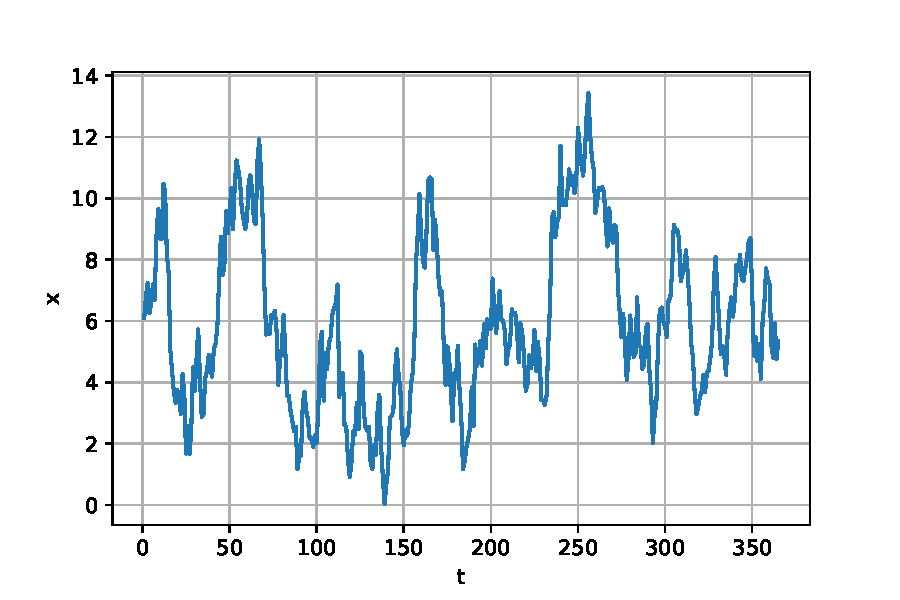
\includegraphics[width=0.5\textwidth]{Data/first.pdf}}
\subfloat[]{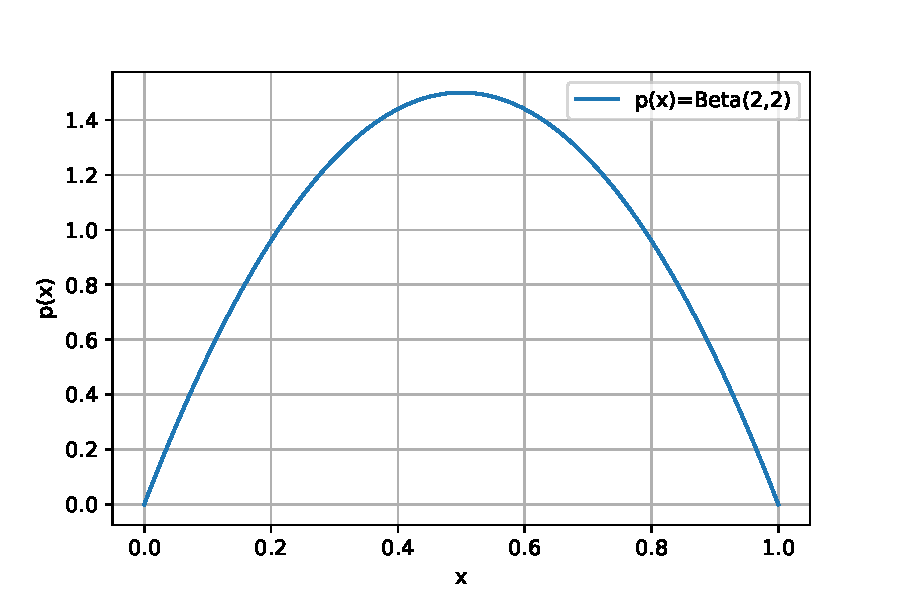
\includegraphics[width=0.5\textwidth]{Data/second.pdf}}\\
\caption{информативный prior}
\end{figure}
{\bf Описание:}\\
\quad
	(a) --- случайное блуждание. Тогда $p(t_{i+1}) \sim N(t_{i+1}|t_{i},\sigma^2)$\\
\quad
	(б) --- информативный prior на параметр в $Be(\theta)$. Проверяем насколько симетрична монетка только что вышедшая с конвейера.\\
	~\\
\end{frame}
%----------------------------------------------------------------------------------------------------------
\begin{frame}{Примеры}
\begin{figure}[h!t]\center
\subfloat[]{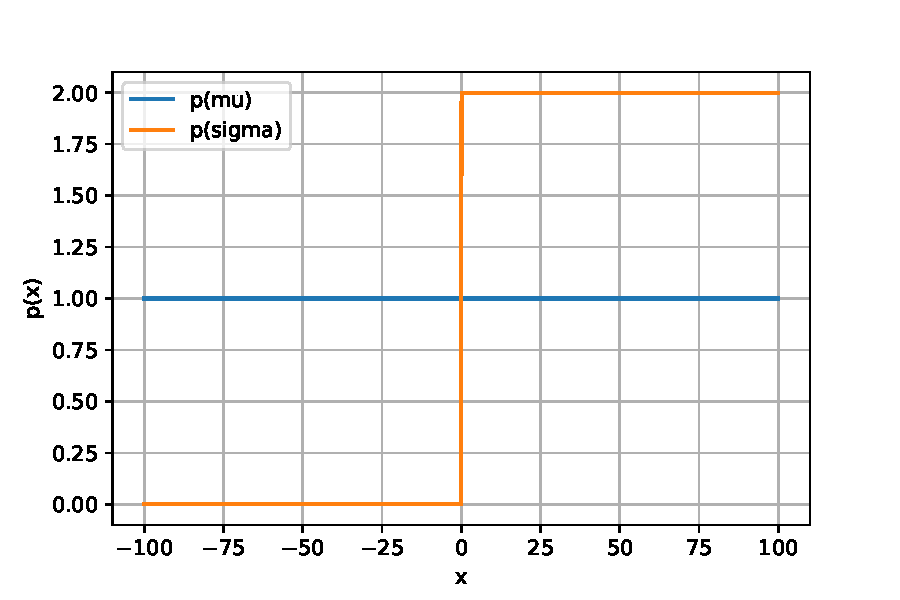
\includegraphics[width=0.5\textwidth]{Data/third.pdf}}
\subfloat[]{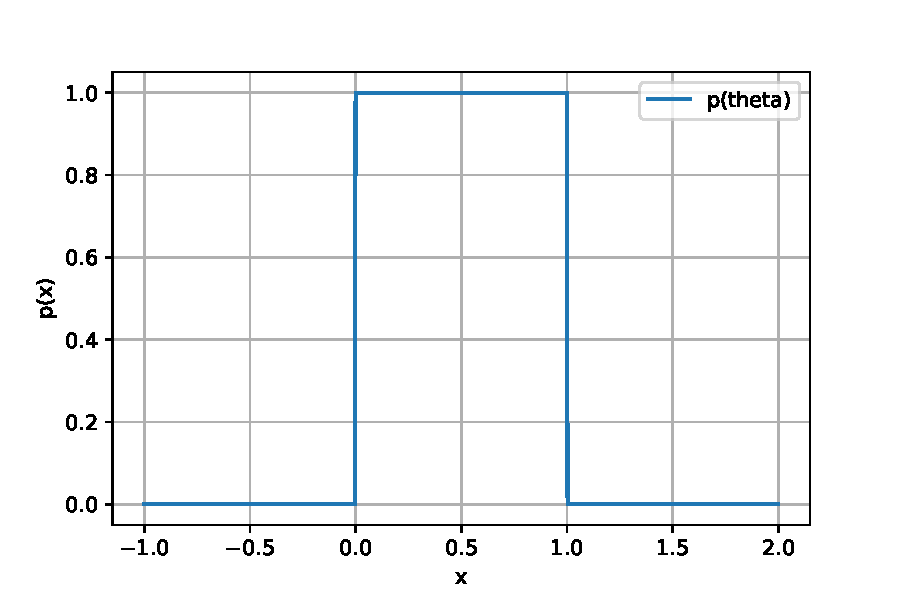
\includegraphics[width=0.5\textwidth]{Data/forth.pdf}}\\
\caption{неинформативный prior}
\end{figure}
{\bf Описание:}\\
\quad
	(a) --- $\mu$ и $\sigma$ параметры нормального распределения\\
\quad
	(б) --- неинформативный prior на параметр в $Be(\theta)$. Заложены только знания о том, что $\theta$ это вероятность.\\
	~\\
\end{frame}
%----------------------------------------------------------------------------------------------------------
\begin{frame}{Improper prior}

{\bf Improper posterior:}\\
\quad
	$x \sim Be(\theta),~p(\theta) = \frac{1}{\theta(1-\theta)} = Beta(0,0) \Rightarrow \int_0^1 p(\theta)d\theta > -\log0 = \infty$\\
\quad
	$p(\theta|x) \propto \theta^{x - 1}(1-\theta)^{-x} \Rightarrow \int_0^1 p(\theta|x)d\theta = \int_0^1 \theta^{x-1}(1-\theta)^{-x}d\theta = \infty$\\
	~\\
{\bf Proper posterior:}\\
\quad
	$x \sim Bin(n, \theta),~ p(\theta) = Beta(0,0)$\\
\quad
	$p(\theta|x) \propto \theta^{x-1}(1-\theta)^{n-x-1} \Rightarrow \int_0^{1}p(\theta|x)=\int_0^1 \theta^{x-1}(1-\theta)^{n-x-1}d\theta \leq$\\
	$\leq_{x\not=n} \int_0^1\theta^{x-1}d\theta =_{x\not=0} \frac{1}{x}$\\
	~\\
{\bf Теорема:}\\
\quad
	Если априорное распределение дискретной(непрерывной) случайной величины собственное распределение, тогда апостериорное распределение всегда(почти всегда) собственное.\\
	 $p(\theta|x) \propto p(x|\theta)p(\theta) \Rightarrow \int p(x|\theta)p(\theta)d\theta = p(x) \leq \sum p(x_i) = $\\
	$=\sum\int p(x_i|\theta)p(\theta)d\theta = \int\sum p(x_i|\theta)p(\theta)d\theta = \int p(\theta)d\theta < \infty$
	~\\
\end{frame}
%----------------------------------------------------------------------------------------------------------
\begin{frame}{Reference prior}
Пусть $p(\theta)$, $p(\theta|x)$ --- априорное и апостериорное распределение некоторого параметра $\theta$, q(x) --- неизвестное распределение наблюдаемой величины $x$\\
~\\
{\bf Определение:}\\
\quad
	$$KL(p) = \mathsf{E}\left[D_{KL}\left(p\left(\theta|x\right)||p\left(\theta\right)\right)\right] \to \max_{p}$$
\quad
	 В некотором смысле мы выбираем такой prior, который является наименее информативным после наблюдения $x$.\\
	~\\
{\bf Альтернативная форма:}\\
\quad
	$KL(p)=\int q(x)\int p(\theta|x)\log\frac{p(\theta|x)}{p(\theta)}d\theta dx = -\int q(x)H(\theta|x)dx + H(\theta)~\textcolor[rgb]{1,0,0}{=}$\\
где $H(x) = -\int p(x)\log p(x)dx$ --- энтропия\\
\quad
	$$\textcolor[rgb]{1,0,0}{=}~-\int p(\theta)\log\left[\frac{p(\theta)}{\sqrt[]{N\mathcal{I}(\theta)}}\right]d\theta = - D_{KL}(p||\mathcal{I}) \to \max_{p} \Rightarrow p(\theta) \propto \sqrt[]{\mathcal{I}(\theta)}$$
	~\\

\end{frame}
%----------------------------------------------------------------------------------------------------------
\begin{frame}{Jeffreys prior}

{\bf Определение:}\\
\quad
$p(\bar{\theta}) \propto \sqrt[]{\det\mathcal{I}(\bar{\theta})} \Rightarrow p(\theta) \propto \sqrt[]{\mathcal{I}(\theta)},~\mathcal{I}(\theta) = -\mathsf{E}\left[\frac{\partial^2 \log L}{\partial^2\theta}\right]$\\
	~\\
	
{\bf Не зависит от параметризации:}\\
\quad
$p(\phi) \propto p(\theta)\left|\frac{\partial\theta}{\partial\phi}\right| \propto \sqrt[]{\mathsf{E}\left[\frac{\partial^2\log L}{\partial\theta^2}\right]\frac{\partial\theta^2}{\partial\phi^2}} =  \sqrt[]{\mathsf{E}\left[\frac{\partial^2\log L}{\partial\phi^2}\right]} = \sqrt[]{\mathcal{I}(\phi)}$\\
	~\\
{\bf Пример использования:}\\
\quad 
Пусть заданы $x \sim Be(\theta)$ и задана параметризация $\phi = \frac{\theta}{1-\theta}$\\
\quad
$\log L(x, \theta) = x\log\theta + (1-x)\log(1-\theta) \Rightarrow \mathcal{I}(\theta) = \frac{1}{\theta(1-\theta)}$\\
\quad
$p(\theta) \propto \sqrt[]{\mathcal{I}(\theta)} \Rightarrow p(\theta|x)\propto \theta^{x-\frac{1}{2}}(1-\theta)^{\frac{1}{2} - x}$\\
\quad
$p(\phi|x) = p(\theta|x)\frac{\partial\theta}{\partial\phi} \propto \textcolor[rgb]{1,0,0}{\frac{\phi^{x-\frac{1}{2}}}{(1+\phi)^2}}$\\
\quad
$\log L(x, \phi) = x\log\phi-\log(1+\phi) \Rightarrow \mathcal{I}(\phi) = \frac{1}{\phi(1+\phi)^2}$\\
\quad
$p(\phi)\propto \sqrt[]{\mathcal{I}(\phi)} \Rightarrow p(\phi|x)\propto \textcolor[rgb]{1,0,0}{\frac{\phi^{x-\frac{1}{2}}}{(1+\phi)^2}}$
	~\\
	
\end{frame}
%----------------------------------------------------------------------------------------------------------
\begin{frame}{Jeffreys prior}

{\bf Распределение Гаусса с $\mu$ как параметром:}\\
\quad
	$p(x|\mu) = \frac{\exp\left(-\frac{(x-\mu)^2}{2\sigma^2}\right)}{\sqrt[]{2\pi\sigma^2}}\Rightarrow p(\mu) \propto \sqrt[]{\mathcal{I}(\mu)} = \sqrt[]{\mathsf{E}\left(\frac{1}{\sigma^2}\right)} = \frac{1}{|\sigma|} \propto 1$\\
	~\\
{\bf Распределение Гаусса с $\sigma$ как параметром:}\\
\quad
	$p(x|\sigma) = \frac{\exp\left(-\frac{(x-\mu)^2}{2\sigma^2}\right)}{\sqrt[]{2\pi\sigma^2}} \Rightarrow p(\sigma) = \sqrt[]{\mathsf{E}\left(\frac{3(x-\mu)^2}{\sigma^4} - \frac{1}{\sigma^2}\right)} = \sqrt[]{\frac{1}{2\sigma^2}}\propto \frac{1}{|\sigma|}$\\
	~\\
{\bf Распределение Пуассона с $\lambda$ как параметром:}\\
\quad
	$p(n|\lambda) = e^{-\lambda}\frac{\lambda^n}{n!} \Rightarrow p(\lambda) = \sqrt[]{\mathsf{E}\left(\frac{n}{\lambda^2}\right)} = \sqrt[]{\frac{1}{\lambda}}$\\
	~\\
	
Во всех 3-х случаях получаем improper prior для $\mu$, $\log|\sigma|$ и $\sqrt[]{\lambda}$.
\end{frame}
%----------------------------------------------------------------------------------------------------------
\begin{frame}{Вывод}

{\bf Информативный \& неинформативный prior:}\\
\quad
	Информативный prior, тот в который вкладываются некоторые знания об наблюдениях.\\
\quad
	Неинформативный prior, использует только общие представления о функции распределения.\\
	~\\
{\bf Собственный \& несобственный prior:}\\
\quad
	Можно использовать improper prior $\Rightarrow$ нужно проверить posterior\\
\quad
	Использовав proper prior $\Rightarrow$ posterior всегда proper\\
	~\\
{\bf Jeffreys prior:}\\
\quad
	Априорное распределение, которое построено на основе максимизации ожидаемого сходства prior и соответствующего ему posterior.
	~\\
\end{frame}
%----------------------------------------------------------------------------------------------------------






\end{document} 